\chapter{Grundlagen}\label{pre}

Wir werden uns in dieser Arbeit hauptsächlich mit einfachen planaren Graphen beschäftigen, also solchen die keine Mehrfachkanten und Schleifen besitzen und für die kreuzungsfreie Zeichnungen, beziehungsweise Einbettungen, in der Ebene existieren. Sei $G = (V,E)$ ein Graph bestehend aus der Menge der Knoten $V$ und der Menge der Kanten $E \subseteq ( \,V \times V ) \,$. Eine Kante $e=(u,v)$ verbindet die beiden Knoten $u$ und $v$. Einen Graphen $G$, definiert als Kombination der Mengen von Knoten und Kanten nennen wir auch einen \textit{kombinatorischen} Graphen. Ein Pfad von $u$ nach $v$ ist eine Folge von Kanten $\{(u,w_1),(w_1,w_2),\ldots,(w_k,v)\} \subset E$ die $u$ und $v$ verbindet. Mit dem Grad deg$(v)$ eines Knoten meinen wir die Anzahl der adjazenten Kanten, der Kanten die $v$ als einen Endpunkt haben.

Eine Einbettung (oder Zeichnung) eines Graphen in der Ebene ist eine Abbildung $m:G\to\mathbb{R}^2$ die die Kanten und Knoten kreuzungsfrei in die Ebene zeichnet. Einen planaren Graphen zusammen mit einer möglichen kreuzungsfreien Einbettung in der Ebene bezeichnen wir als \textit{ebenen Graphen}. Für einen ebenen Graphen können wir, zusätzlich zu den Knoten und Kanten, auch die Menge der Gebiete (engl. faces) $F$ betrachten, das heißt die durch die Kanten und Knoten begrenzten Regionen in der Ebene. Wir bezeichnen das unbeschränkte Gebiet als das \textit{äußere} Gebiet. Wir können den Begriff der Einbettung von $G$ auch etwas weiter fassen und mit diesem nur die Definition der Menge der Gebiete $F$ von $G$ und eines äußeren Gebietes $f_{aus} \in F$ meinen, sodass mindestens eine planare Zeichnung mit diesen Gebieten existiert. Wir nennen dies auch eine \textit{kombinatorische} Einbettung. Die kombinatorische Einbettung bildet eine Äquivalenzklasse aller möglichen Zeichnungen von $G$. In ihr enthalten sind alle Zeichnungen von $G$ deren Gebiete (inklusive dem Äußeren) denen der kombinatorischen Einbettung entsprechen. Wir werden im Verlauf der Arbeit, wenn wir von Einbettung reden, manchmal eine spezifische Zeichnung und manchmal ihre Äquivalenzklasse meinen, die Bedeutung sollte sich jedoch aus dem Kontext ergeben.

\section{Geradlinige Dreiecks-Darstellungen (SLTRs)}

Wir werden uns in dieser Arbeit mit Möglichkeiten auseinandersetzten, geradlinige Dreiecks-Darstellungen für planare Graphen zu finden. Die englische Bezeichnung der geradlinigen Dreiecks-Darstellungen lautet straight line triangle representation, kurz SLTR. Die nächste Definition formalisiert diese Darstellung.

\begin{definition}[SLTR]\label{defsltr}
Eine Zeichnung eines ebenen Graphen $G$ wird \textit{SLTR} genannt falls gilt:
\begin{itemize}
\item[S1] Alle Kanten sind Segmente von Geraden.
\item[S2] Alle Gebiete, inklusive dem Äußeren, sind nicht-degenerierte Dreiecke.
\end{itemize}
\end{definition}

\begin{figure}[h]
	\centering
  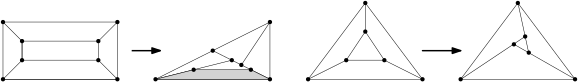
\includegraphics[width=0.95\textwidth]{sltr-example.png}
	\caption{Links einer der beiden 3-zusammenhängenden Graphen mit acht Knoten ohne SLTR und rechts ein Graph mit einer möglichen SLTR.}
\end{figure}

Für die weiteren Betrachtungen ist es nützlich die drei Knoten $\{a_1,a_2,a_3\}$, die das äußeren Gebiet berühren, gesondert zu betrachten. Wir nennen sie die \textit{Aufhängungen} von $G$. Die Knoten $a_1,a_2$ und $a_3$ sind dann die designierten Ecken des äußeren Gebietes einer möglichen SLTR. Einen Graphen zusammen mit einem äußeren Gebiet und festen Aufhängungen als Paar zu behandeln ist sinnvoll, wie in Beispiel \ref{bsp1} zu sehen sein wird.

\begin{example}\label{bsp1}
Es existieren planare Graphen, von denen manche Einbettungen SLTRs zulassen, andere jedoch nicht. Betrachten wir den planaren Graphen mit zehn Knoten aus Abbildung \ref{10_example}. Mit rot und grün sind die beiden Gebiete markiert die jeweils einmal als das äußere Gebiet festgelegt wurden. Die kombinatorische Einbettung auf der rechten Seite lässt zu dieser Wahl des äußeren Gebietes keine SLTR zu. Das nicht dreieckige Gebiet ist grau eingefärbt. Zu Auswahl auf der linken Seite existiert hingegen eine. Dies ist der kleinste 3-zusammenhängende kombinatorische Graph, der diese Eigenschaft hat.

\begin{figure}[h]
\centering
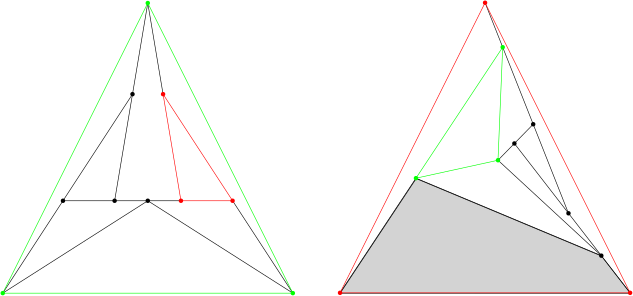
\includegraphics[width=0.7\textwidth]{10_example.png}
\caption{Zwei topologische Einbettungen des (kombinatorisch) gleichen planaren Graphen, wobei die linke keine SLTR zulässt.}
\label{10_example}
\end{figure}

\end{example}

Bevor wir zur ersten Proposition kommen werden wir die Klasse der planaren Graphen, die wir betrachten wollen etwas weiter einschränken. Dabei hilft uns die nächste Definition.

\begin{definition}[intern-k-zusammenhängend]\label{int_3_con}
Ein Graph $G$ ist zusammenhängend falls für alle Knoten $u,v$ ein Pfad von $u$ nach $v$ existiert. $G$ ist \textit{k-zusammenhängend}, falls er nach der Entfernung von $k-1$ beliebigen Knoten weiterhin zusammenhängend ist. Sei $G$ eben mit den Aufhängungen $\{a_1,a_2,a_3\}$, weiter sei $a_\infty$ ein zusätzlicher Knoten eingefügt im äußeren Gebiet. Dann ist $G$ \textit{intern k-zusammenhängend}, falls $G+a_\infty\coloneqq(V\cup\{a_\infty \},E\cup \{(a_1,a_\infty),(a_2,a_\infty),(a_3,a_\infty)\})$ k-zusammenhängend ist.
\end{definition}

Die nächste Präposition enthält eine erste notwendige Bedingung für die Existenz von geradlinigen Dreiecksdarstellungen (SLTRs).

\begin{proposition}\cite[Proposition 1.2]{af13}
Sei $G$ ein ebener Graph mit den Aufhängungen $\{a_1,a_2,a_3\}$ als äußere Ecken einer SLTR. Weiter gelte für alle Knoten $v\in V \backslash \{a_1,a_2,a_3\}$ deg$(v) \geq 3$. Dann ist $G$ intern-3-zusammenhängend.
\end{proposition}

\begin{proof}
Sei $\Delta$ die SLTR von $G=(V,E)$. Angenommen es existiert eine Menge $U \subseteq V$ in $G$ mit $|U| = 2$, deren Entnahme $G$ in nicht zusammenhängende Komponenten trennt. Wir werden zeigen, dass jeder Teil von $G\backslash U$ eine der Aufhängungen enthält und somit $G + a_\infty$ nicht von $U$ getrennt wird. Da $G$ intern-3-zusammenhängend ist können nur die Aufhängungen $a_i$ Grad zwei haben. Sei $K$ eine der Komponenten von $G\backslash U$. Betrachte $K\cup U$ als induzierten Teilgraphen von $G$. Falls $K\cup U$ ein Pfad ist, also nur Knoten von Grad zwei oder eins enthält, dann kann nur $K=\{a_i\}$ gelten.

Falls $K\cup U$ kein Pfad ist, betrachte die konvexe Hülle von $U \cup K$ in $\Delta$. Mindestens drei der Ecken von $U \cup K$ haben Außenwinkel grösser als $\pi$ (an diesen Ecken befinden sich Knoten aus $U \cup K$). Zwei dieser Winkel können an den Knoten aus $U$ liegen, aber der dritte muss ein Winkel sein, der schon in $\Delta$ existiert. Es handelt sich somit um eine Aufhängung.
\end{proof}

\begin{remark}
Für innere Knoten von Grad 2 in einer SLTR müssen die beiden angrenzenden Winkel gerade sein. Somit kann man diese Knoten durch eine gerade Kante zwischen ihren Nachbarn ersetzen und den resultierenden Graphen betrachten. Knoten von Grad eins können nicht existieren, da sie nicht aus dem Rand eines Dreiecks liegen können. Wir werden somit von nun an nur intern-3-zusammenhängende Graphen mit Aufhängungen betrachten, da alle anderen Graphen, die eine SLTR zulassen, auf diese reduziert werden können.
\end{remark}

Für 3-zusammenhängende planare Graphen mit mehr als drei Knoten ist die kombinatorische Einbettung nach Hassler Whitney bis auf Wahl des äußeren Gebietes eindeutig \cite{whitney32}. Zusammen mit der nächsten Proposition definiert somit die Wahl von Aufhängungen $\{a_1,a_2,a_3\}$, die in mindestens einem gemeinsamen Gebiet liegen, ein eindeutiges äußeres Gebiet $f_{aus}$.

\begin{proposition}
Sei $G$ ein planarer 3-zusammenhängender Graph und $\{a_1,a_2,a_3\} \subset V$. Dann existiert höchstens ein Gebiet $f$, das adjazent zu $a_1,a_2,a_3$ ist.
\end{proposition}

\begin{proof}
Angenommen es existieren zwei Gebiete $f,f'$ die $a_1,a_2$ und $a_3$ enthalten. Dann berühren sich diese Gebiete an mehr als einer Kante (vergleiche Abbildung \ref{3_con_uni} links). Im grauen Gebiet müssen Knoten liegen, da $G$ 3-zusammenhängend ist. Wenn wir aber nun $a_2$ und $a_3$ entfernen, dann teilen wir $G$ in zwei nicht zusammenhängende Gebiete. Es kann somit nur ein Gebiet $f$ geben, in welchem die $a_1,a_2$ und $a_3$ liegen.
\end{proof}

\begin{figure}
	\centering
  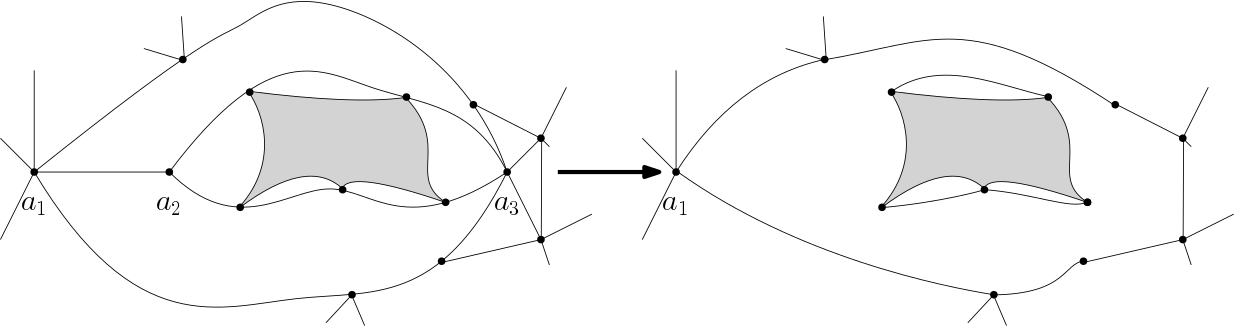
\includegraphics[width=0.95\textwidth]{3_conn_uni.png}
	\caption{Die entnehme der Knoten $a_2$ und $a_3$ trennt $G$, was zu einem Wider- spruch zum 3-Zusammenhang führt.}
	\label{3_con_uni}
\end{figure}

\begin{remark}
Wir könnten uns somit für 3-zusammenhängende planare Graphen auf die Wahl von Aufhängungen $\{a_1,a_2,a_3\}$ beschränken. Für eine kombinatorische Einbettung folgt dann ein eindeutiges äußeres Gebiet $f_{aus}$. Für nur intern-3-zusammenhängende planare Graphen gilt dies nicht. Wir betrachten somit im Folgenden ebene Graphen mit Aufhängungen $\{a_1,a_2,a_3\}$ im äußeren Gebiet.
\end{remark}

Mit den Fragen, welche notwendigen und hinreichenden Bedingungen für die Existenz von SLTRs gelten und welche algorithmischen Ansätze man bei der Suche nach einer spezifischen Darstellung verfolgen kann, werden wir uns in den nächsten beiden Kapiteln auseinandersetzen. Zuvor werden in diesem Kapitel noch einige Konzepte eingeführt, die notwendig sind, um der Argumentation zu folgen.

\section{Schnyder Woods}\label{sw}
Betrachten wir einen ebenen Graphen mit Aufhängungen $a_1,a_2,a_3$. Anschaulich handelt es sich bei einem Schnyder Wald um drei Aufspannende Bäume $T_1,T_2,T_3$, sodass jeder der Bäume $T_i$ zu seiner Wurzel $a_i$ hin gerichtet ist. Jede der Kanten wird mindestens von einem der Bäume genutzt und Kanten können von zwei der drei Bäume gleichzeitig genutzt werden.

Schnyder Wälder, im weiteren nach der englischen Bezeichnung \textit{Schnyder Woods}, wurden zuerst von Walter Schnyder eingeführt \cite{schnyder89}. Es handelt sich die um eine Färbung und Orientierung der inneren Kanten einer Triangulierung. Sie dienten der Betrachtung der von planaren Graphen induzierten Ordnungen. In einer weiteren Arbeit wurden mit ihrer Hilfe geradlinige und konvexe Einbettungen Triangulierungen auf einem $(|V|-2)\times(|V|-2)$ Gitter erzeugt \cite{schnyder90}.

Wir wollen hier die Verallgemeinerung auf 3-zusammenhängende planare Graphen durch Felsner und die zu ihnen in Bijektion stehenden Schnyder Labelings einführen \cite{felsner01}. Wir orientierten uns dabei an einem Lehrbuch von Felsner \cite{felsner04}. Für den Rest dieses Kapitels sei $G$, wenn nicht weiter spezifiziert, ein 3-zusammenhängender ebener Graph mit Aufhängungen $\{a_1,a_2,a_3\}$.

\begin{definition}[Schnyder Woods]\label{def_sw}
Ein Schnyder Wood ist eine Orientierung und Beschriftung der Kanten von $G$ mit den Labeln 1, 2 und 3\footnote{Es wird davon ausgegangen, dass die Label zyklisch sortiert sind, sodass $i+1$ und $i-1$ immer definiert sind.} (alternativ wird hier auch oft rot, grün und blau genutzt), unter Berücksichtigung der folgenden Regeln:
\begin{itemize}
\item[W1] Jede Kante ist entweder in eine oder zwei Richtungen orientiert. Falls sie bigerichtet ist, haben beide Richtungen unterschiedliche Label.
\item[W2] An jeder Aufhängung  $a_i$ existiert eine nach außen gerichtete Halbkante\footnote{Eine Halbkante ist eine Kante mit nur einem Endpunkt.} mit Label i. 
\item[W3] Jeder Knoten $v$ hat Ausgangsgrad eins in jedem Label. Um $v$ existieren im Uhrzeigersinn eine Auskante mit Label 1, null oder mehr eingehende Kanten mit Label 3, eine Auskante mit Label 2, null oder mehr  eingehende Kanten mit Label 1, eine Auskante mit Label 2 und null oder mehr  eingehende Kanten mit Label 2.
\item[W4] Es existiert kein inneres Gebiet mit einem gerichteten Zykel in einer Farbe als Rand.
\end{itemize}
\end{definition}

\begin{figure}[h]
	\centering
  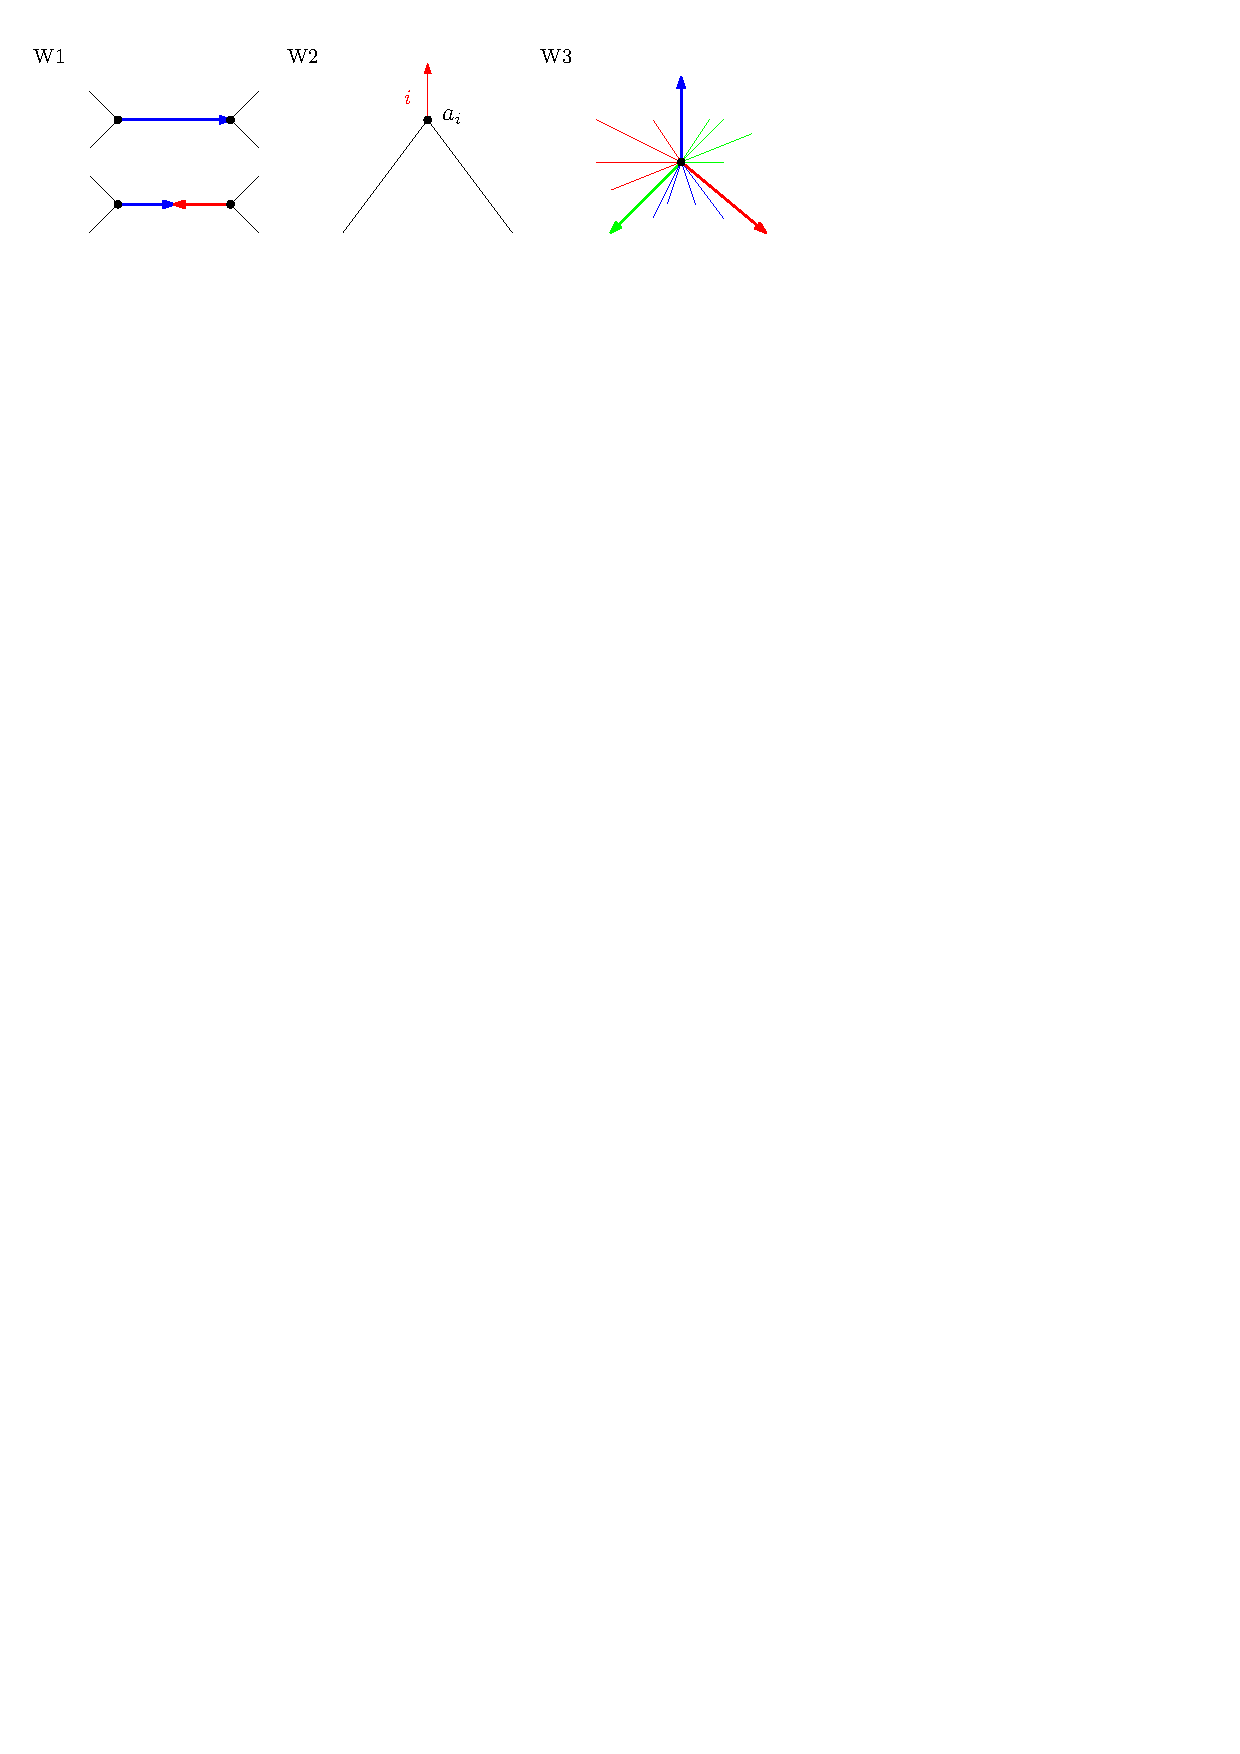
\includegraphics[width=0.9\textwidth]{schnyder_wood_def.pdf}
  \caption{Illustration der ersten drei Bedingungen für Schnyder Woods.}
\end{figure}

Analog zu den Schnyder Woods, kann man Schnyder Labelings definieren, die zu diesen in Bijektion stehen. Hier betrachten wir nicht zuerst die Kanten eines planaren Graphen sondern die Winkel an den Knoten.

\begin{definition}[Schnyder Labeling]\label{def_sl}
Ein Schnyder Labeling ist eine Beschriftung der Winkel von $G$ mit den Labeln 1, 2 und 3 (oder rot, grün und blau) unter Berücksichtigung der folgenden Regeln:
\begin{itemize}
\item[L1] Um jedes innere Gebiet bilden die Label im Uhrzeigersinn nichtleere Intervalle von 1en, 2en und 3en. Am äußeren Gebiet gilt dies gegen den Uhrzeigersinn.
\item[L2] Um jeden inneren Knoten bilden die Label im Uhrzeigersinn nichtleere Intervalle von 1en, 2en und 3en.
\item[L3] An den Aufhängungen $a_i$ haben die äußeren Winkel die Label i-1 und i+1 im Uhrzeigersinn mit der Halbkante dazwischen. Die inneren Winkel haben das Label i.
\end{itemize} 
\begin{figure}[h]
	\centering
  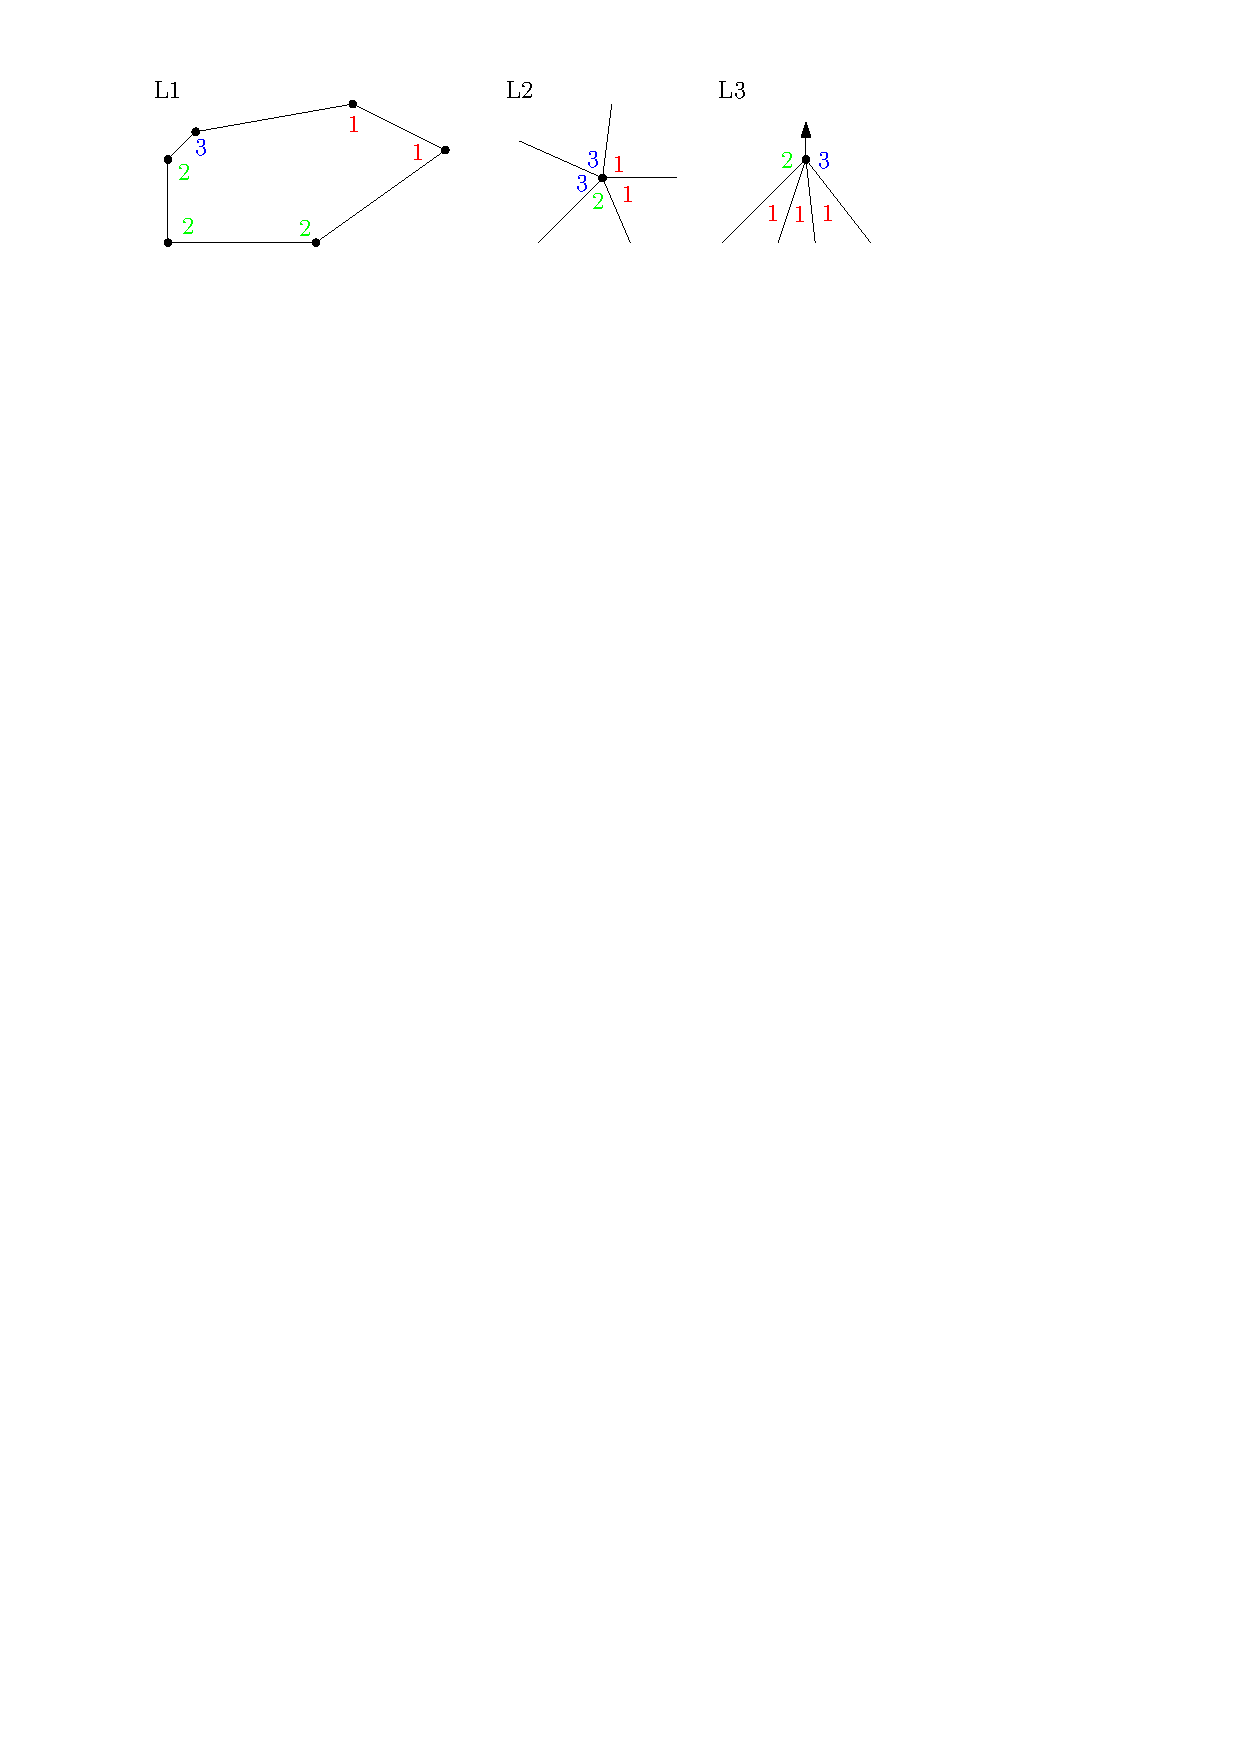
\includegraphics[width=0.9\textwidth]{schnyder_label_def.pdf}
   \caption{Illustration der drei Bedingungen für Schnyder Labelings.}
\end{figure}
\end{definition}

In Abbildung \ref{schnyder_bij} wird eine Verbindung zwischen Schnyder Woods und Schnyder Labelings illustriert. Das nächste Lemma folgt aus den Bedingungen L1 und L2.

\begin{lemma}\label{lem_sl}
Sei G ein ebener, intern-3-zusammenhängender Graph mit den Aufhängungen $a_1,a_2,a_3$ und einem Schnyder Labeling. Dann beinhalten die vier Winkel entgegen dem Uhrzeigersinn an jeder Kante die Label 1, 2 und 3. Somit hat jede Kante einen der beiden Typen in Abbildung \ref{schnyder_bij}.
\end{lemma}

\begin{figure}[h]
	\centering
  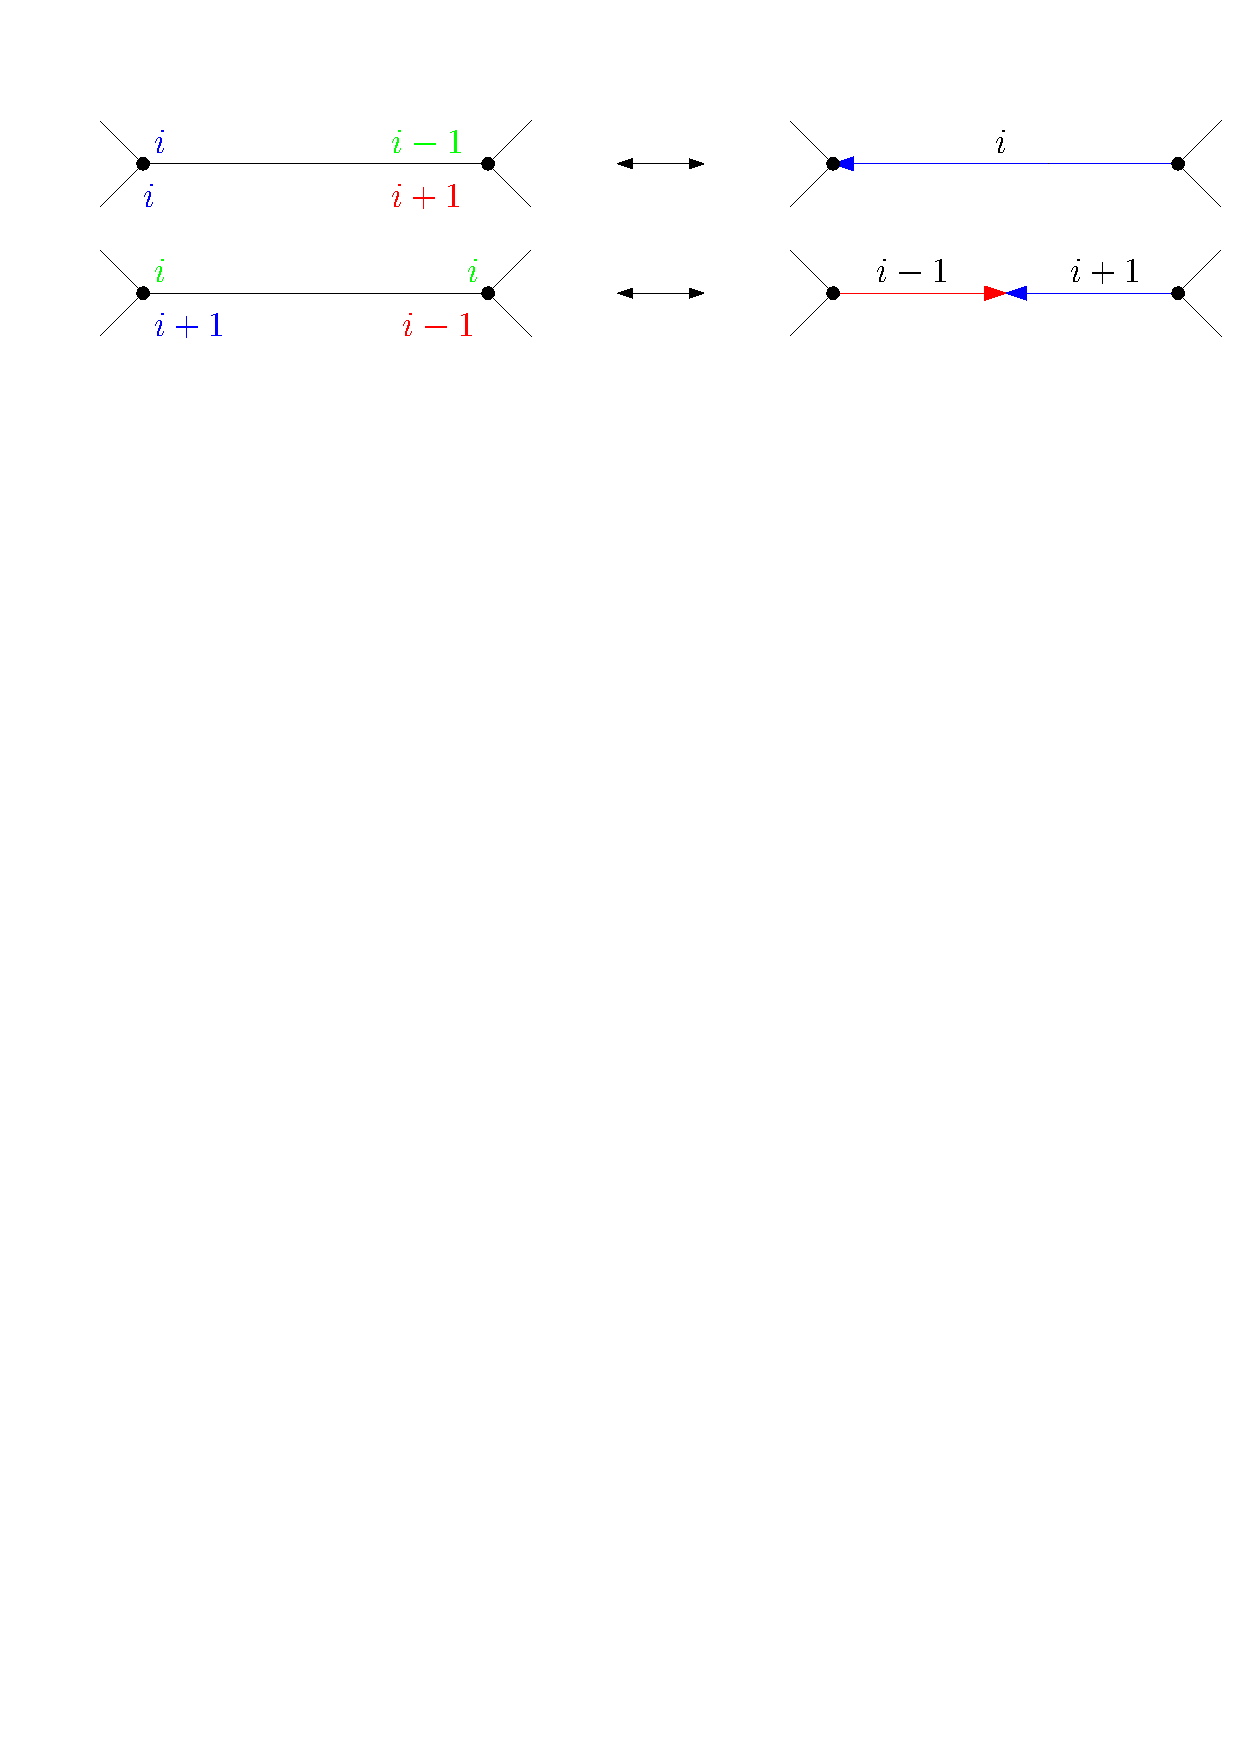
\includegraphics[width=0.9\textwidth]{schnyder_bij.pdf}
	\caption{Bijektion zwischen Schnyder Wood auf der rechten und Schnyder Labeling auf der linken Seite.}
	\label{schnyder_bij}
\end{figure}

\begin{theorem}\label{theo_schnyder_bij}
Sei G ein ebener, intern-3-zusammenhängender Graph mit den Aufhängungen $a_1,a_2,a_3$. Der in Abbildung \ref{schnyder_bij} dargestellte Zusammenhang erzeugt eine Bijektion zwischen Schnyder Woods und Schnyder Labelings auf $G$.
\end{theorem}

Dies macht es möglich, wenn für Darstellung und Verständnis sinnvoll, zwischen den beiden Strukturen hin und her zu wechseln. So kann es im Verlauf dieser Arbeit vorkommen, dass wir vom einen schreiben, aber implizit Eigenschaften des anderen meinen. Für die von uns im Folgenden betrachteten Graphen existiert mindestens ein Schnyder Wood. Dies belegt das nächste Theorem nach Ezra Miller \cite[Theorem A]{miller02}.

\begin{theorem}
Sei $G$ ein ebener Graph mit Aufhängungen $\{a_1,a_2,a_3\}$. $G$ ist genau dann intern-3-zusammenhängend, wenn ein Schnyder Wood auf $G$ mit den Ecken $\{a_1,a_2,a_3\}$ existiert.
\end{theorem}

\subsection{Einbettungen via Schnyder Woods}\label{face_counting}

Es existieren einige Anwendungen von Schnyder Woods in Bezug auf Einbettungen. Wie schon erwähnt, bezieht sich eines der ersten Resultate auf die konvexe Einbettung auf einem Gitter. Das im Folgenden skizzierte \textit{face-counting} nach Felsner (deutsch: Gebiete zählen), erzeugt eine Einbettung auf einem kleineren Gitter als nach Schnyder \cite{felsner01}. Betrachte $G$ mit einem Schnyder Wood $T_1,T_2,T_3$. Es handelt es sich bei den Bäumen $T_i$ um gerichtete Bäume mit Wurzeln in $a_i$ \cite[Korollar 2.5]{felsner04}. Von jedem Knoten $v$ aus existierten also eindeutige Pfade $P_i(v)$ zu den Aufhängungen $a_i$. Jeweils zwei der Pfade von $v$ zu den Aufhängungen haben $v$ als einzigen gemeinsamen Knoten \cite[Lemma 2.4]{felsner04}. Wir können somit zu jedem Konten $v$ drei Regionen $R_i$ definieren, die jeweils von den Pfaden $P_{i-1}(v)$ und $P_{i+1}(v)$ und dem äußeren Gebiet eingegrenzt werden\footnote{Ein Beispiel für diese Regionen findet sich in Abbildung \ref{face_counting} auf der rechten Seite.}. In jeder dieser Regionen können wir nun die eingeschlossenen Gebiete von $G$ zählen. Durch das Zählen der Gebiete in den Regionen zu $v$ lässt sich eine konvexe Zeichnung von $G$ erzeugen.

Hierzu ordnet man jedem Knoten $v$ seinen \textit{Gebietsvektor} $(v_1,v_2,v_3)$ zu, wobei $v_i$ die Anzahl der inneren Gebiete in $R_i(v)$ beschreibt. In Abbildung \ref{face_counting} sind auf der rechten Seite die Regionen von $v$ eingefärbt. Seien $\alpha_1 = (0,1),\alpha_2 = (1,0)$ und $\alpha_3 = (0,0)$ die äußeren Ecken unserer Zeichnung. Sie entsprechen ebenfalls den Bildern der Aufhängungen von $G$. Die Position der inneren Knoten ergibt sich nun durch die Funktion 
$$\mu: V \to \mathbb{R}^2,v\mapsto v_1\alpha_1 + v_2\alpha_2+v_3\alpha_3.$$ 

\begin{theorem}[Theorem 2.7 \cite{felsner04}]
Sei G ein ebener Graph mit einem Schnyder Wood $\sigma$ und den Aufhängungen $a_1,a_2,a_3$. Sei $(v_1,v_2,v_3)$ der, unter Berücksichtigung von $\sigma$ berechnete, Gebietsvektor von $v \in V$, mit $ v_i = \text{Anzahl der Gebiete in }R_i(v).$ Dann ist die Zeichnung $\mu(G)$ konvex.
\end{theorem}

Die mit diesen Koordinaten erzeugte Einbettung von $G$ ist planar, konvex und passt, falls $G$ 3-zusammenhängend ist, auf ein $(|F|-1)\times(|F|-1)$-Gitter \cite[Korollar 2.8]{felsner04}. Sie hat noch eine weitere Eigenschaft, die später von Nutzen sein wird und die in der nächsten Proposition festgehalten ist.  Dies ist in Abbildung \ref{face_counting} in der Mitte skizziert.

\begin{figure}
	\centering
  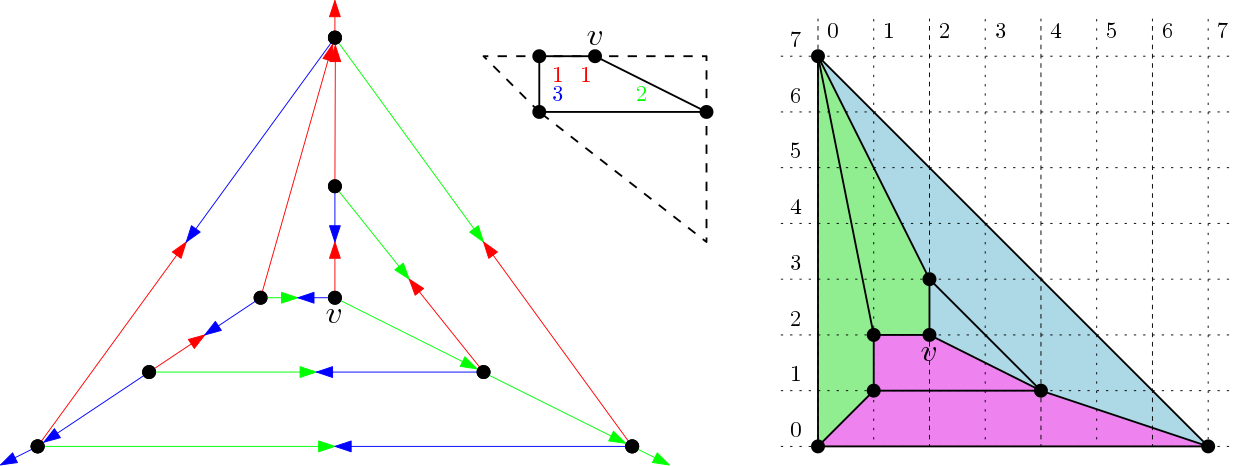
\includegraphics[width=1\textwidth]{face_counting.png}
	\caption{Eine Schnyder Wood auf $G$ und die durch face-counting erhaltene Einbettung von $G$. Die eingefärbten Gebiete sind die Regionen die den Gebietsvektor $(v_1,v_2,v_3)$ ergeben. In der Mitte ist W5 illustriert.}
	\label{face_counting}
\end{figure}

\begin{proposition}\label{w5}
Sei G ein ebener Graph mit einem Schnyder Wood $\sigma$ und den Aufhängungen $a_1,a_2,a_3$. Für $\mu(G)$, die durch face-counting erzeugte Einbettung von $G$, gilt:
\begin{itemize}
\item [W5] Die Knoten eines inneren Gebietes werden auf die Seiten eines Dreiecks mit den Seiten $c_i(\alpha_{i-1}-\alpha_{i+1})$ mit passenden Konstanten $c_i$ abgebildet. Im inneren dieses Dreiecks befinden sich keine Knoten. Die Winkel im Inneren des Gebietes an den Knoten auf der Seite $c_i(\alpha_{i-1}-\alpha_{i+1})$ haben Label $i$ im Schnyder Labeling.
\end{itemize}
\end{proposition}

\section{$\alpha$-Orientierungen}\label{alpha_orientations}

Für den Algorithmus in Kapitel \ref{main_algo} führen wir nun eine weitere zu Schnyder-Woods und Labelings in Bijektion stehende Struktur auf Graphen ein und folgen dabei weiter Felsners Lehrbuch \cite{felsner04}.

\begin{definition}[$\alpha$-Orientierung]
Sei $G=(V,E)$ ein ungerichteter Graph und $\alpha:V\mapsto\mathbb{N}$ eine Funktion auf $G$. Eine $\alpha$\textit{-Orientierung} ist eine Orientierung der Kanten von $G$, sodass der Ausgangsgrad\footnote{Der Ausgangsgrad eines Knoten $v$ entspricht der Anzahl der adjazenten Kanten von $v$, die von $v$ weg gerichtet sind.} eines jeden Knoten $\alpha(v)$ entspricht, dass heißt $$\text{outdeg}(v) = \alpha(v).$$
\end{definition}

Um von $\alpha$-Orientierungen zu Schnyder Woods zu gelangen müssen wir Primal-Dual Graphen betrachten, die mit den nächsten beiden Definitionen eingeführt werden.

\begin{definition}[schwacher dualer Graph]
Sei $G$ ein ebener Graph. Wir definieren $G^*$, den \textit{schwachen dualen Graphen} von $G$. $G^*$ hat einen (Gebiets-)Knoten für jedes innere Gebiet von $G$. Für jede innere Kante in $G$ fügen wir eine Kante zwischen den beiden (Gebiets-)Knoten $f,f'$ in $G^*$ ein, die adjazent zu dieser Kante in $G$ sind.
\end{definition}

\begin{definition}[Primal-Dual Graph]
Betrachte einen ebenen Graphen $G$ und seinen schwacher dualen Graphen $G^*$. Der \textit{Primal-Dual Graph} $G+G^*$ ist eine Vereinigung der Graphen $G$ und $G^*$. Wenn wir $G$ und $G^*$ übereinander legen, dann kreuzen sich jeweils eine Kante aus $G$ und eine aus $G^*$. An so einer Kantenkreuzung fügen wir in $G+G^*$ einen Knoten ein und verbinden ihn mit den adjazenten Knoten aus $G$ und $G^*$. Die Menge der Knoten von $G+G^*$ besteht aus Knoten-Knoten (Knoten in $G$), Kanten-Knoten (an den Kreuzungen) und Gebiets-Knoten (Knoten in $G^*$). Kanten in $G+G^*$ existieren, sowohl zwischen inzidenten Kanten und Knoten, als auch Kanten und Gebieten in $G$. Hinzu kommen Halbkanten von den Kanten-Knoten und Knoten-Knoten am äußeren Gebiet von $G$. Wenn wir einen Knoten $f_\infty$ für das äußere Gebiet hinzufügen und die Halbkanten zu diesem verlängern spricht man vom \textit{Abschluss} von $G+G^*$. Ein Beispiel ist in Abbildung \ref{alpha_ex} a) zu sehen.

\end{definition}

Wir trennen bei der Erzeugung jede Kante in zwei Teile. Die Kanten-Knoten auf er einen und die Knoten-Knoten und Gebiets-Knoten auf der anderen Seite bilden Bipartition. Somit sind $G+G^*$ und sein Abschluss bipartit. Das folgende Theorem liefert eine Bijektion zwischen den Schnyder Woods auf $G$ und einer bestimmten $\alpha$-Orientierung auf dem Abschluss von $G+G^*$, die wir $\alpha_s$ nennen \cite[Propositionen 2.13, 2.14]{felsner04}.

\begin{figure}
	\centering
	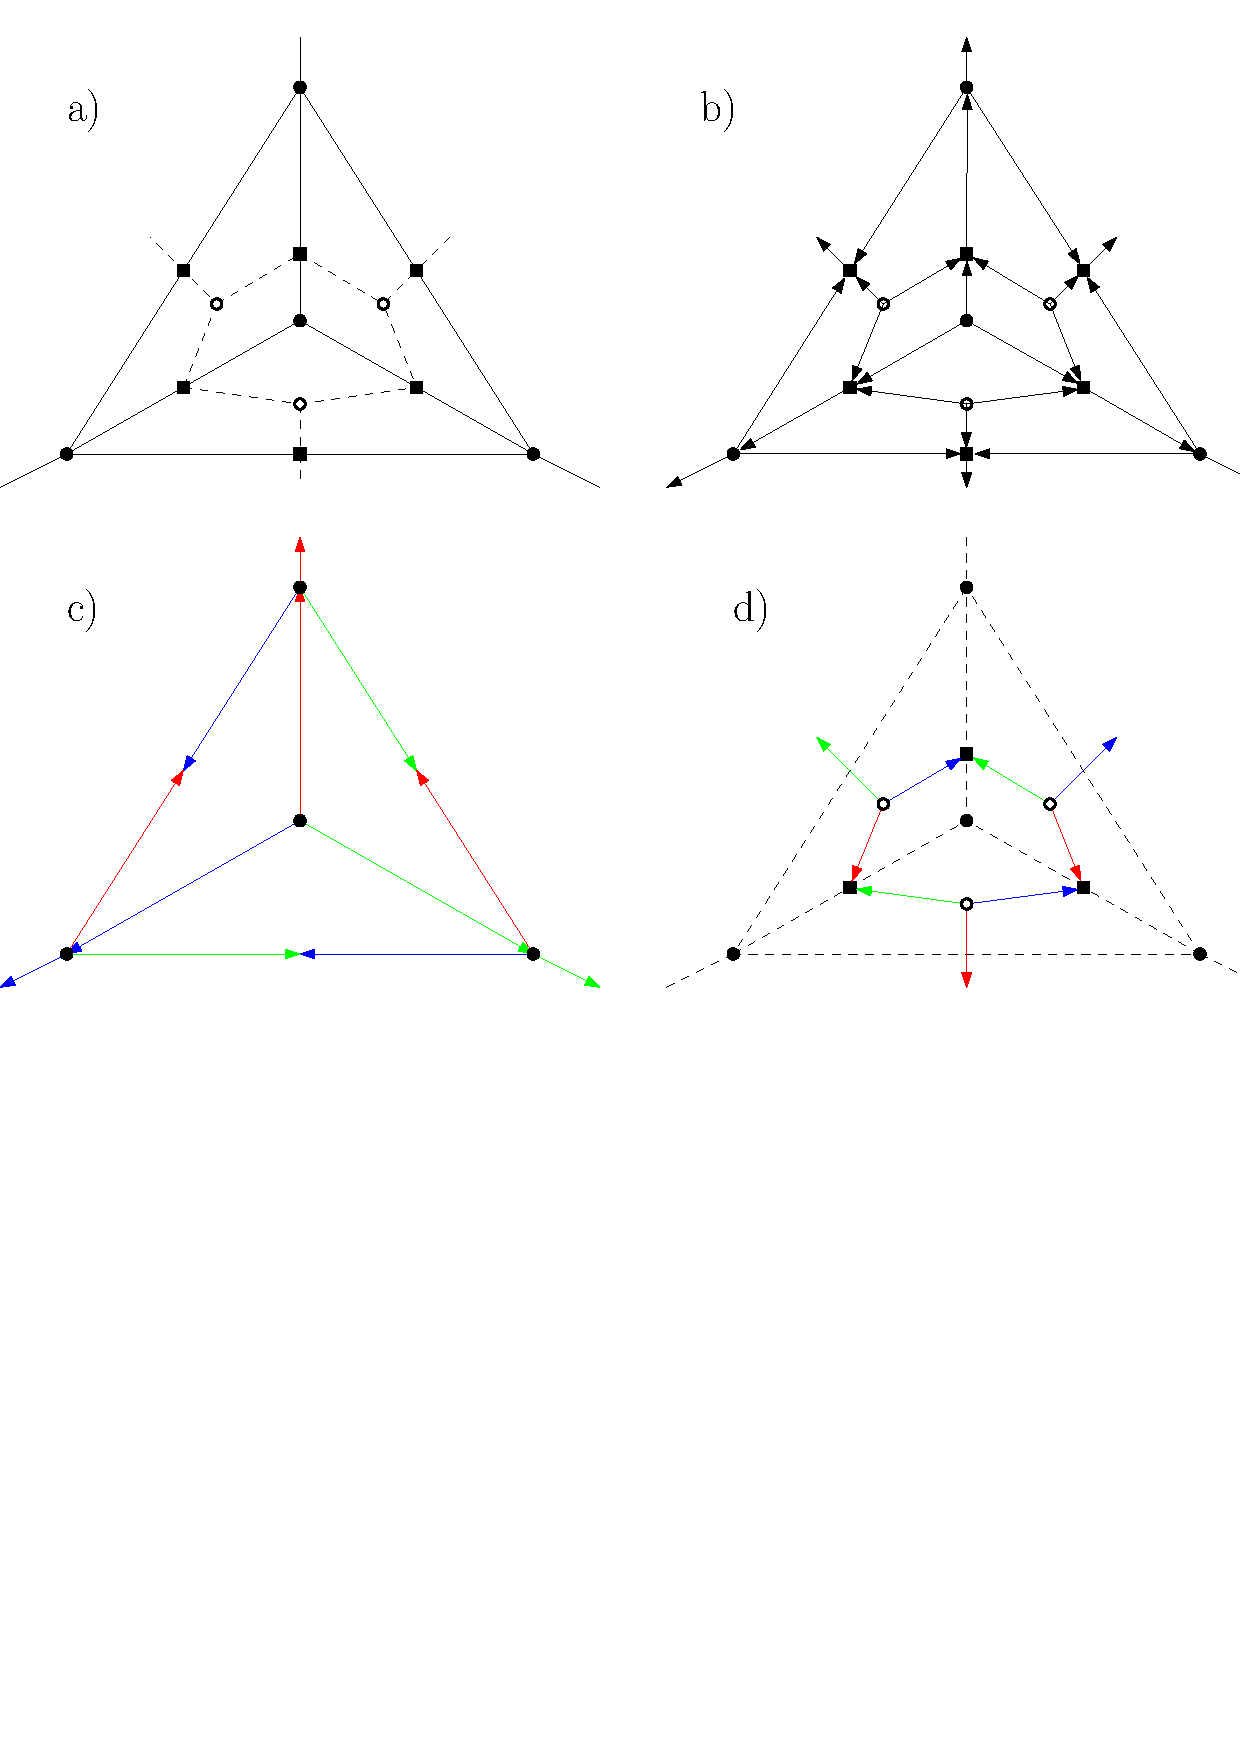
\includegraphics[width=0.8\textwidth]{alpha_ex.pdf}
  \caption{a) Der Primal-Duale Graph $K_4+K_4^*$. b) Mit einer $\alpha_s$-Orientiertung und c) den zugehörigen Schnyder Woods auf $K_4$ d) und $K^*_4$. }
  \label{alpha_ex}
\end{figure}

\begin{theorem}\label{alpha_bij}
Sei $G$ ein ebener Graph mit Aufhängungen $\{a_1,a_2,a_3\}$, dann stehen die folgenden Strukturen in Bijektion:
\begin{itemize}
\item [A1] Die Schnyder Woods auf $G$.
\item [A2] Die Schnyder Woods auf dem (schwachen) dualen Graphen $G^*$.
\item [A3] Die $\alpha_{s}$-Orientierungen des Abschlusses von $G+G^*$ mit $\alpha_s(v) = \alpha_s(f) = 3$ für jeden Knoten-Knoten $v$ und Gebiets-Knoten $f$,  $\alpha_s(e) = 1$ für jeden Kanten-Knoten $e$ und  $\alpha_s(f_\infty) = 0$.
\end{itemize}
\end{theorem}

Wir erklären kurz die erhaltene Bijektion von A1 und A2 zu A3. Angenommen wir haben ein Paar in Bijektion stehender Schnyder Woods $\sigma,\sigma^*$ auf $G$ und $G^*$. Die von $\sigma$ und $\sigma^*$ induzierte Orientierung der Kanten von $G+G^*$ ist eine $\alpha_s$-Orientierung. 

Angenommen wir haben eine $\alpha_s$-Orientierung auf dem Abschluss von $G+G^*$. Sie induziert die Orientierung der Kanten der resultierenden Schnyder Woods $\sigma$ und $\sigma^*$. Wir müssen jedoch noch die Label bestimmen. Dies erfolgt mit Hilfe der Gerader Pfad Regel. 

\begin{description}
\item[Gerader Pfad Regel:] Beginnen wir auf einer beliebigen Kante von $G+G^*$. Wenn wir einen Kanten-Knoten $e$ betreten, dann verlassen wir diesen auf der gegenüberliegenden Seite (wir folgen der zugrunde liegenden Kante in $G$ bzw. $G^*$). Wenn wir einen Knoten-Knoten oder Gebiets-Knoten $v$ betreten und über eine Kante kommen die zu $v$ orientiert ist, dann laufen wir auf der gegenüberliegenden, von $v$ weg orientierten Kante, weiter\footnote{Es existieren genau drei von $v$ weg orientierte Kanten und wir wählen die von uns aus gesehen Mittlere.} (vergleiche Abbildung \ref{straight_path} a). Falls wir $v$ über eine von $v$ weg orientierte Kante betreten, dann hängt unsere Wahl der Auskante von der Orientierung am letzten Kanten-Knoten $e$\footnote{Wir betreten Kanten-Knoten nur über zu diesen hin orientierte Kanten.} ab. Falls dort die Auskante auf der rechten Seite liegt, wählen wir jetzt die rechte\footnote{Falls wir $v$ durch eine von $v$ weg orientierte Kante betreten, dann bleiben noch zwei andere übrig.} von $v$ weg orientierte Kante, sonst die linke (vergleiche Abbildung \ref{straight_path} b). Falls wir $a_\infty$ erreichten laufen wir nicht weiter. 
\end{description}

\begin{figure}
	\centering
	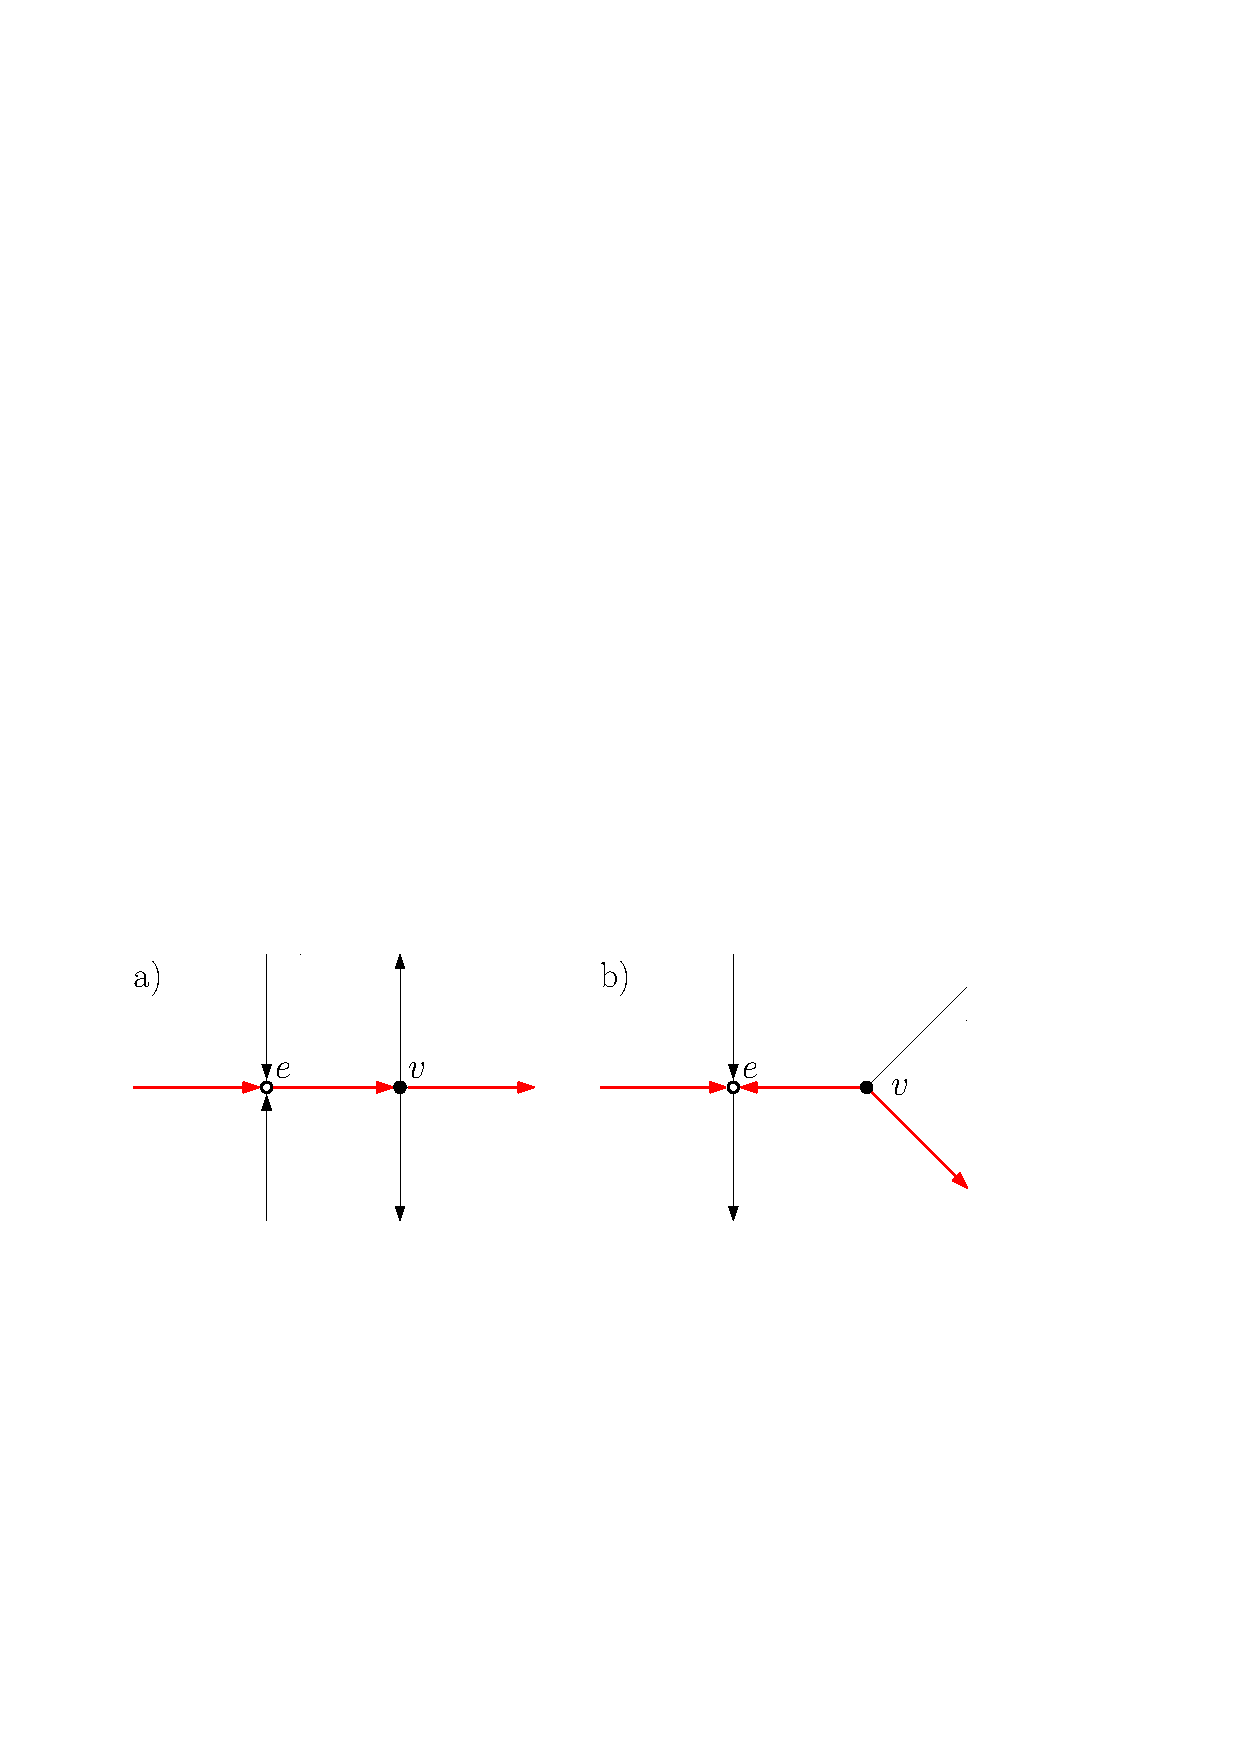
\includegraphics[width=0.7\textwidth]{straight_path.pdf}
  \caption{Die zwei Fälle der Gerader Pfad Regel beim Betreten eines Knoten $f$ aus $G$ oder $G^*$. In rot der gewählte und somit eingefärbte Pfad.}
  \label{straight_path}
\end{figure}

Betrachten wir einen Pfad nach der Regel, der mit einer gerichteten Kante $e \in G+G^*$ beginnt. Dann endet er in $a_\infty$ \cite[Lemma 15]{felsner01}. Der letzte passierte Knoten muss nun entweder eine der Aufhängungen von $G$ oder $G^*$ sein. Wir Färben den Pfad in der Farbe dieser Aufhängung. Die so erhaltene Orientierung und Färbung auf den Kanten von $G$ und $G^*$ entspricht zwei in Bijektion stehenden Schnyder Woods $\sigma$ und $\sigma^*$ \cite{felsner01}.

\section{Gerichtetes-Multi-Fluss-Problem}\label{dir_multi_flow}

Wir werden in Kapitel \ref{main_algo} einen gerichteten Graphen $\mathcal{N}$ auf Basis von $G$ konstruieren, sodass ein maximaler Fluss $\varphi$ einer SLTR von $G$ entspricht. Es gibt sehr viele unterschiedliche Arten von Flussproblemen. So kann man zum Beispiel Graphen mit nur einem Paar von Quellen und Senken oder mit jeweils mehreren betrachten und die Kanten können gerichtet oder ungerichtet sein. Im Fall von mehreren Quellen und Senken werden diese normalerweise als Paare $s_i,t_i$ gehandhabt und es wird gefordert, dass insgesamt Fluss $\varphi_i$ mit Stärke $d_i \in \mathbb{R}_+$ von $s_i$ zu $t_i$ fließt. Als zusätzliche Einschränkung haben die Kanten $e$ maximale Kapazitäten $c(e) \in \mathbb{R}_+$ die nicht überschritten werden können. Für jede Kante muss also gelten $\varphi(e) \leq c(e)$. Wir werden uns in Kapitel \ref{main_algo} mit einem Fluss der folgenden Form befassen.

\begin{definition}[Gerichtetes-Multi-Fluss-Problem]\label{def_multi_flow}
Sei $\mathcal{N}=(V,E)$ ein gerichteter Graph, im Weiteren auch Netzwerk genannt, mit den Kapaziäten $c:E\mapsto\mathbb{R}_{+}$, Paaren von ausgezeichneten Knoten $\{(s_1,t_1), ... ,(s_n,t_n)\}\subset V \times V$ und positiven Bedarfen $\{d_1, ... ,d_n\} \in \mathbb{R}_+^n$. Dann bilden die Funktionen $\varphi_i: E \to \mathbb{R}_+^{|E|}$ einen zulässigen Fluss $\varphi=(\varphi_1, ... ,\varphi_n)$ auf $\mathcal{N}$, falls
\begin{itemize}
\item[M1] $\forall (u,v) \in E : \sum_{i=1}^{n}{\varphi_i(u,v)} \leq c(u,v) $
\item[M2] $ \forall u \neq s_i,t_i : \sum_{w \in V} \varphi_i(u,w) - \sum_{w \in V} \varphi_i(w,u) $
\item[M3] $ \forall s_i : \sum_{w \in V} \varphi_i(s_i,w) - \sum_{w \in V} \varphi_i(w,s_i) = d_i $
\item[M4] $ \forall t_i : \sum_{w \in V} \varphi_i(w,s_i) - \sum_{w \in V} \varphi_i(s_i,w) = d_i $
\end{itemize}
Mit $|\varphi_i|$ bezeichnen wir die Menge des Flusses von $s_i$ nach $t_i$.
\end{definition}

\begin{definition}
Wir nennen die Kantenmenge $S \subseteq \mathcal{N}_G(E)$ einen \textit{Schnitt} in $\mathcal{N}_G$, falls seine Entnahme alle Paare $\{s_i,t_i\}$ trennt. Die Kantenmenge $S$ ist ein \textit{minimaler Schnitt}, falls für alle anderen Schnitte $\tilde{S}$ gilt: $c(S) \leq c(\tilde{S})$.
\end{definition}

Es folgen zwei bekannte Resultate für den Fall $n=1$. Das erste Theorem stammt von Ford und Fulkerson \cite{ff09}.

\begin{theorem}[Max-Flow Min-Cut]
Der maximale zulässige Fluss auf einem Netzwerk $\mathcal{N}$ mit einer Quelle und Senke entspricht der Kapazität eines minimalen Schnittes.
\end{theorem}

Ein maximaler Fluss lässt sich zum Beispiel mit dem Edmonds-Karp-Algorithmus in polynomineller Zeit bestimmen \cite[Theorem 8.15]{korte12}. Ein direktes Resultat folgt nach Danzig und Fulkerson \cite{ff09}

\begin{theorem}[Ganzzahliger Fluss]\label{theo_int_flow}
Sei $\mathcal{N}$ ein Netzwerk mit einer Quelle und einer Senke und ganzzahligen Kapazitäten $c:E\mapsto\mathbb{N}$. Sei $\tilde{\varphi}$ ein nicht ganzzahliger Fluss auf $\mathcal{N}$. Dann existiert auch ein Fluss $\varphi$, mit $|\tilde{\varphi}| = |\varphi|$, sodass der Fluss $\varphi$ auf allen Kanten ganzzahlig ist.
\end{theorem}

Nach dem Max-Flow Min-Cut Theorem impliziert die Kapazität eines minimalen Schnittes im eindimensionalen Fall die Stärke eines maximalen Flusses. Für $n=2$ existieren für ungerichtete Graphen analoge Aussagen nach T. Chiang Hu \cite{hu}. Für diese Arbeit wäre im Folgenden jedoch der Fall $n=2$ für gerichtete Graphen interessant. Es existieren jedoch keine analogen Aussagen zum Max-Flow Min-Cut Theorem, welche für Gerichtete-Multi-Fluss-Probleme mit mindestens zwei Quellen und Senken aussagekräftig wären, sondern nur Schranken und Annäherungen \cite{leighton99}.

Im eindimensionalen Fall mit ganzzahligen Kapazitäten $c:E\mapsto\mathbb{N}$ impliziert die Existenz eines zulässigen Flusses nach Theorem \ref{theo_int_flow} die Existenz einer ganzzahligen Lösung, sowohl für gerichtete als auch für ungerichtete Graphen. Die Unterscheidung zwischen ganzzahligen und nicht ganzzahligen Flüssen ist relevant, da das Entscheidungsproblem, ob ein solcher Fluss existiert, im mehrdimensionalen Fall in unterschiedlichen Komplexitätsklassen liegt. Die Berechnung eines nicht (zwangsläufig) ganzzahligen zulässigen Flusses $\varphi$ auf $\mathcal{N}$ ist für den ein- und mehrdimensionalen Fall über eine LP-Formulierung in polynomieller Zeit möglich \cite[Theorem 4.18]{korte12}. Für ganzzahlige Lösungen gilt dies selbst in einfachen Fällen im Allgemeinen nicht und somit kann auch keine analoge Formulierung zu Theorem \ref{theo_int_flow} existieren.

\begin{theorem}[\cite{even75}]\label{np_hard}
Die Berechnung einer ganzzahligen Lösung eines Gerichtetes-Multi-Fluss-Problems auf einem Netzwerk $\mathcal{N}$ mit zwei Paaren von Quellen und Senken $\{(s_1,t_1),(s_2,t_2)\}$ und Kapazitäten $c:E\mapsto\mathbb{N}$ ist sogar dann NP-schwer, wenn $\mathcal{N}$ keine gerichteten Zykel enthält.
\end{theorem}

NP-schwere Entscheidungsprobleme lassen sich nicht in polynomieller Zeit lösen. Somit existiert kein im Allgemeinen gültiger deterministischer polynomieller Algorithmus zur Berechnung eines zulässigen ganzzahligen Flusses für ein Gerichtetes-Multi-Fluss-Problem für den Fall $n\geq2$.


